\chapter{Interfaz y resultados finales}
\label{cap:Interfaz y resultados finales}

PyQt, wxPython y Kivy son opciones populares para la implementación de interfaces gráficas, cada una con sus propias ventajas y desventajas.

PyQt es conocido por su completo conjunto de widgets, lo que te permite crear interfaces gráficas complejas y altamente personalizadas. Sin embargo, puede tener una curva de aprendizaje más pronunciada debido a su complejidad y sintaxis más verbosa.

Por otro lado, wxPython ofrece una sintaxis más simple y fácil de entender, lo que puede ser beneficioso si estás empezando o prefieres un enfoque más directo. Aunque tiene menos widgets y funcionalidades avanzadas que PyQt, sigue siendo una opción sólida con una comunidad activa que proporciona soporte.

Kivy destaca por su diseño adaptable, diseñado para crear aplicaciones con interfaces gráficas que funcionan en una amplia gama de dispositivos. Utiliza un lenguaje de marcado declarativo que permite definir la interfaz de usuario de manera intuitiva y separada del código Python. Sin embargo, puede tener menos documentación y recursos disponibles en comparación con PyQt y wxPython.

Sin embago, y pese a las grandes funcionalidades de todas estas alternativas nos hemos decantado por hacer una interfaz con telegram desarrollando nuestro propio chatbot usando rasa. 

Para configurarlo, en primer lugar hay que ejecutar el programa mibot.py estando en telegram en la conversaa conversación de telegram el comando /start para comenzar la conversación y ya. 


Con esto la interfaz se ve de la siguiente forma: 

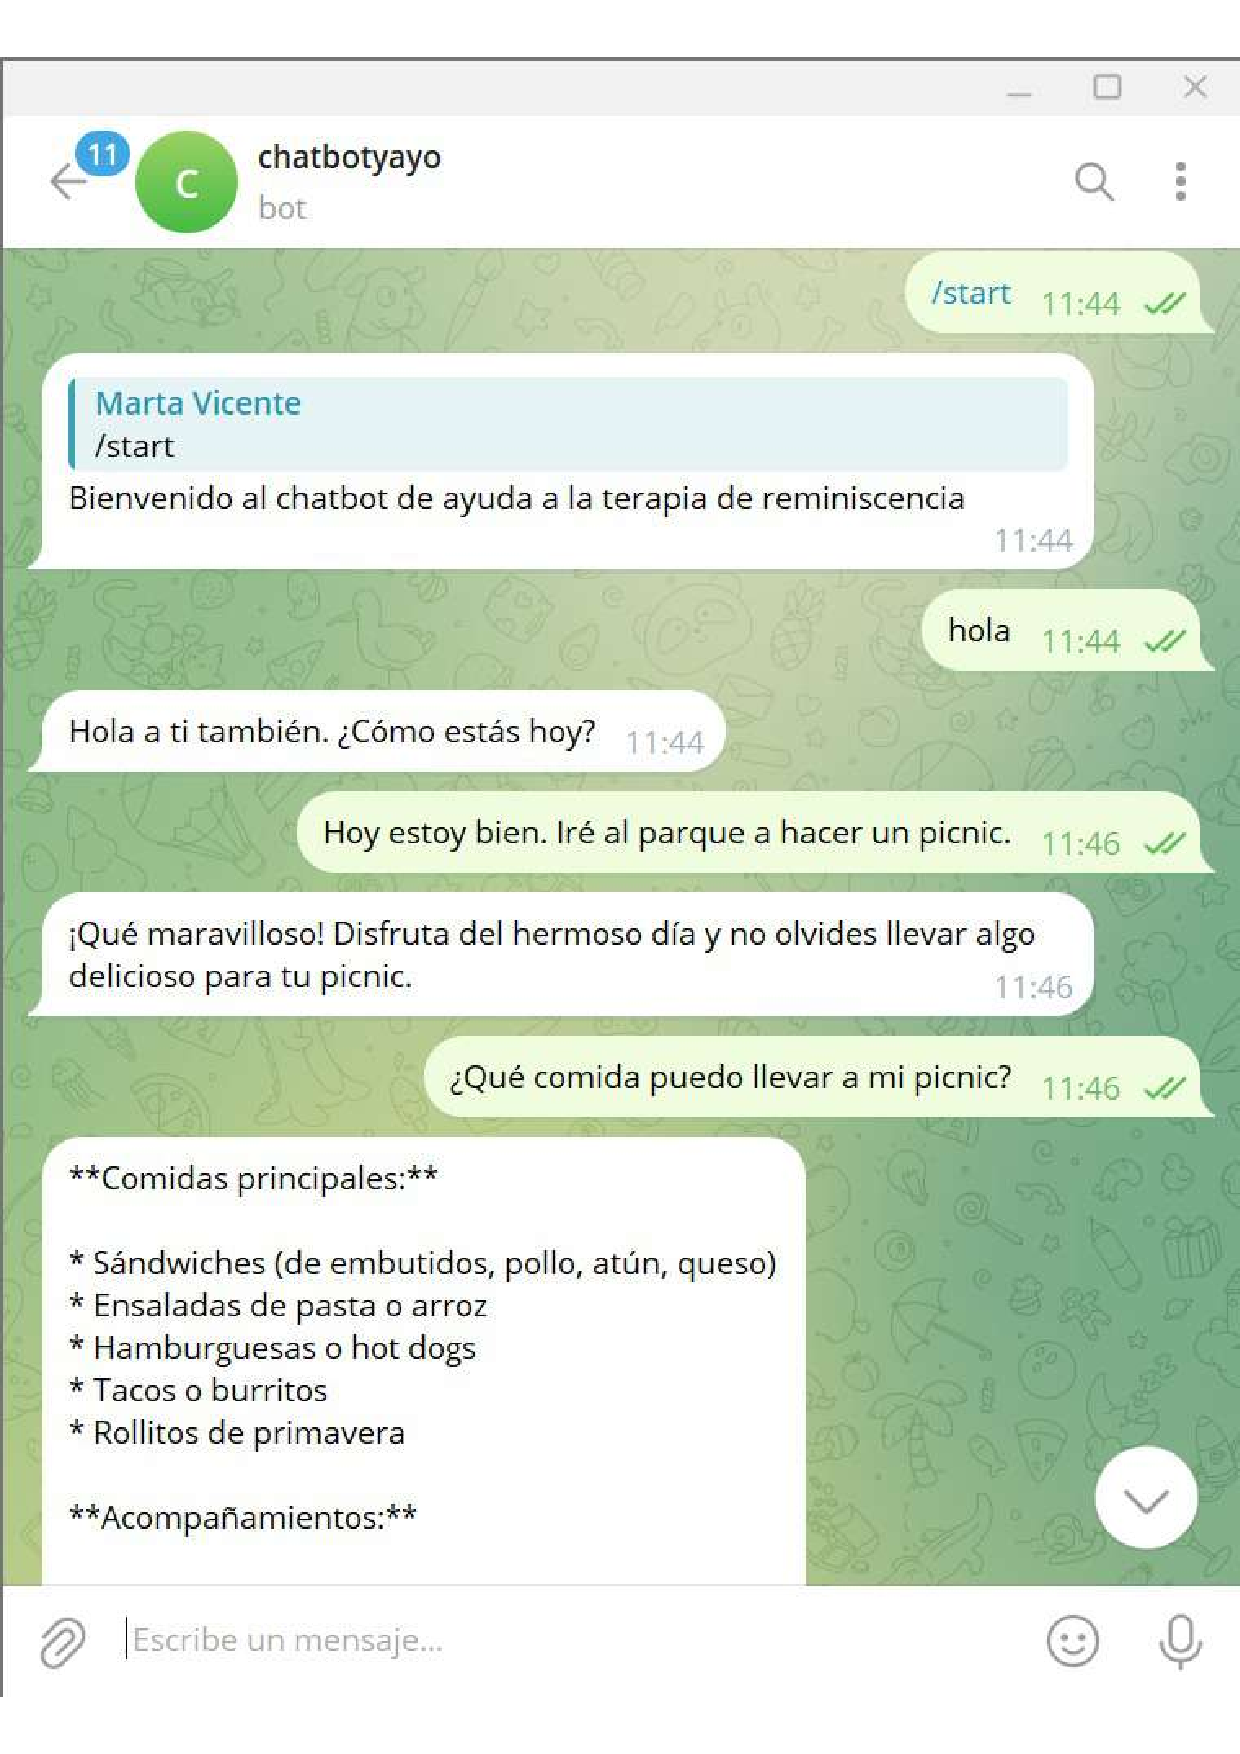
\includegraphics[width=0.5\textwidth]{Imagenes/telegram1}


Para desarrollar el chatbot de telegram me he decantado por usar la interfaz de telegram para la cuál se necesita la API de Rasa. Las principales ventajas que ofrece esta herramienta es la facilidad del manejo de la interfaz pues telegram es una herramienta muy conocida con la que los terapeutas pueden estar más familiarizados. Además, esto nos permite también usar la versión del chatbotyayo para móvil. 

Para crear está interfaz hay que: 
1. Instalar rasa
2. Instalar telegram 
2. Obtener una api de rasa
4. crear un nuevo chatbot desde telegram con @botFather
5. Enviar a tu chatbot el comando /start

Una vez seguidos todos estos pasos ya puedes comenzar a interactuar con la API de rasa. 


